\documentclass{article}

\usepackage{amsmath, amsthm, amssymb, amsfonts}
\usepackage{thmtools}
\usepackage{graphicx}
\usepackage{setspace}
\usepackage{geometry}
\usepackage{float}
\usepackage{hyperref}
\usepackage[utf8]{inputenc}
\usepackage[english]{babel}
\usepackage{framed}
\usepackage[dvipsnames]{xcolor}
\usepackage[most]{tcolorbox}
\usepackage{minted}
\usepackage{enumitem}
\usepackage{subcaption}
\usepackage{csquotes}

\usepackage{indentfirst}

\usepackage[export]{adjustbox} % Align images

\colorlet{LightGray}{White!90!Periwinkle}
\colorlet{LightOrange}{Orange!15}
\colorlet{LightGreen}{Green!15}

\newcommand{\HRule}[1]{\rule{\linewidth}{#1}}

\newtcbtheorem[auto counter,number within=section]{code}{Código}{
  colback=LightOrange!20,
  colframe=LightOrange,
  colbacktitle=LightOrange,
  fonttitle=\bfseries\color{black},
  boxed title style={size=small,colframe=LightOrange},
}{code}

\setstretch{1.2}
\geometry{
  textheight=22.5cm,
  textwidth=13.75cm,
  top=2.5cm,
  headheight=12pt,
  headsep=25pt,
  footskip=30pt
}

% ------------------------------------------------------------------------------

\begin{document}

% ------------------------------------------------------------------------------
% Cover Page and ToC
% ------------------------------------------------------------------------------
\begin{center}
  \begin{figure}
    
\includegraphics[scale = 0.3, left]{img/IST_A.eps} % IST logo
    \end{figure}
  \LARGE{ \normalsize \textsc{} \\
  [2.0cm] 
  \LARGE{ \LARGE \textsc{Aprendizagem}} \\
  [1cm]
  \LARGE{ \LARGE \textsc{LEIC IST-UL}} \\
  [1cm]
  \HRule{1.5pt} \\
  [0.4cm]
  \LARGE \textbf{\uppercase{Relatório - Merit Prize Challenge}}
  \HRule{1.5pt}
  \\ [2.5cm]
  }
\end{center}

\begin{flushleft}
  \textbf{\LARGE Grupo 10:}
\end{flushleft}

\begin{center}
  \begin{minipage}{0.7\textwidth}
      \begin{flushleft}
        \large Gabriel Ferreira \\
        \large  Irell Zane
      \end{flushleft}
  \end{minipage}%
  \begin{minipage}{0.3\textwidth}
      \begin{flushright}
        \large 107030\\
        \large 107161
      \end{flushright}
  \end{minipage}
\end{center}

\begin{center}
  \vspace{4cm}
  \date \large \bf  2024/2025 -- 1st Semester, P1
\end{center}

\setcounter{page}{0}
\thispagestyle{empty}
\renewcommand{\thesection}{\Roman{section}}

\newpage

% ------------------------------------------------------------------------------
% Content
% ------------------------------------------------------------------------------




%We began by loading the the required dataset, making a 70\%-30\% train-test split, and scaling the data using a \texttt{StandardScaler}.
\begin{enumerate}

  \item \textit{Perform logistic regression and indicate the accuracy.}

\begin{table}[H]
    \centering
    \begin{tabular}{ccc}
        &Testing Accuracy & Training Accuracy \\ \hline
        StandardScaler &98.25\% & 98.74\% \\
        Unscaled &97.66\% & 95.98\%
    \end{tabular}
    \label{tab:log-accuracy}
\end{table}

  \item \textit{Perform EM clustering on the training data set with different number k of clusters. Evaluate
  the quality of the clusterings using Silhouette. Is the number of clusters correlated with the
  quality of clustering? Which is the optimal k?}

We used \texttt{scikit-learn}'s \texttt{GaussianMixture} model to perform EM
clustering on the breast cancer dataset features. An evaluation of the clustering quality was made
using each solution's silhouette for numbers of clusters ranging from 2 to 10, see Figure \ref{fig:silhouette-score}.

\begin{figure}[H]
  \centering
  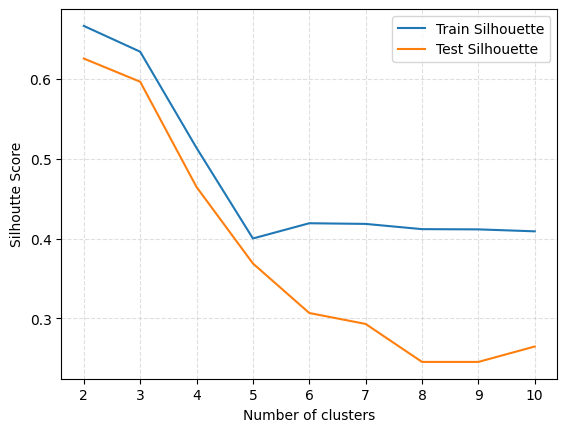
\includegraphics[width=0.5\linewidth]{img/Silhouettes.png}
  \caption{Silhouette of different EM clustering solutions.}
  \label{fig:silhouette-score}
\end{figure}

According to the Silhouette score, there is a trend of declining clustering
quality as the number of clusters increases in the EM clustering solution.
We can also see an increase in the gap in the Silhouette scores
between the classifications of the testing and training samples as the number
of clusters increases, suggesting a deterioration of the generalization
capacity of the clustering solution.

According to these results, the optimal $k$ is $k=2$ with a silhouette score
of 0.626 for the testing sample, and 0.667 for the training sample.

  \item \textit{Map the test set into probability values of the k-clusters. If you have a data point represented
  by a vector of dimension d, you will map it into a vector of dimension:}

  \centering \texttt{prob=em\_model.predict\_proba(X)}

  \raggedright 

  \item \textit{Perform logistic regression on the mapped data set with the labels of the original test set.
  Indicate now the accuracy. Is there a relation between the number of clusters, the cluster
  evaluation and the accuracy of the logistic regression model?}

We mapped the dataset to the cluster probabilities of the different clustering 
solutions and performed logistic regression on these transformed features.

\begin{figure}[H]
  \centering
  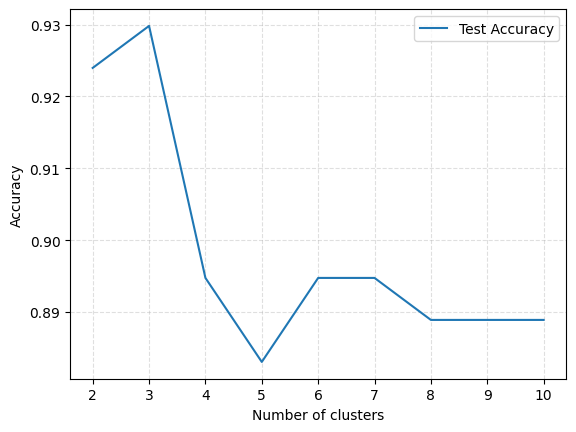
\includegraphics[width=0.5\linewidth]{img/EMProbMapAccuracy.png}
  \caption{Silhouette of different EM clustering solutions.}
  \label{fig:em-accuracy}
\end{figure}

Upon analyzing the relationship between the number of clusters 
($k$) and both performance metrics - the Silhouette scores and
Logistic Regression accuracy on the mapped dataset - we can see
that there is a notable relation: For low numbers of clusters,
such as 2 and 3, both metrics show high values, and as the $k$
increases, there is a sharp decline in both the silhouette score
and the classification accuracy of the logistic model, which
seem to follow the same trajectory, suggesting that a higher
quality of clustering, as measured by the Silhouette score, is
conducive to a better logistic regression model.

Using $k=2$ or $k=3$ the EM algorithm effectively serves as a
dimensionality reduction technique, transforming the original
high-dimensional feature space (30 features) into a lower
dimensional feature space, while maintaining a high accuracy
on the logistic regression model.

The accuracy for the model that used clustering with $k=2$
was $92.4\%$.


  \item \textit{Train an RBF network using the clustering with optimal k from 2).}

A typical RBF Network looks like this:
\begin{enumerate}
    \item Input layer with the dimension of an observation
    \item Hidden layer with the dimension of the number of clusters
    \item Output layer with a single neuron
\end{enumerate}

Before training an RBF network we need to choose an Radial Basis Function.
A Radial Basis Function is any function that depends on the distance,
the most commonly used is the Gaussian, which should be appropriate for EM
clustering:
\begin{equation}
  \phi_k(x)=\phi_k(d(x,c_k))=exp(-\gamma \cdot d(x,c_k)^2)
\end{equation}
Since we are dealing with EM Clusters, we want to measure the distance between the point of the observation and the distribution of cluster 1 and 2, the distance between a point and a distribution is the Mahalanobis distance:
\begin{equation}
  d(x,c_k)^2=(x-\mu)^T\Sigma_k^{-1}(x-\mu)
\end{equation}
So our Radial Basis Function ends up like so:
\begin{equation}
  \phi_k(x)=exp(-\gamma \cdot (x-\mu)^T\Sigma_k^{-1}(x-\mu))
\end{equation}
As in 'Machine Learning: A Journey to Deep Learning'$^{\cite{journey}}$,
we thought the $\gamma$ should be $\frac{1}{2}$; However when this was
tried, the network would always make the same prediction regardless of
the input. This was quite unexpected, we speculated that this was a float
underflowing issue, arising from the negative exponent being too large
resulting into loss of information, but it seems more plausible
that the model was unable to learn when the activation values
were of very different scales and mostly near zero. Thus we plotted
the Accuracy against the Gamma to decrease the exponent and, after tuning 
this hyperparameter, settled on $\gamma = 0.015$ (maximizing training accuracy), see Figure
\ref{fig:gamma-tuning}, resulting in a test accuracy of 92.4\%.
\begin{figure}[H]
    \centering
    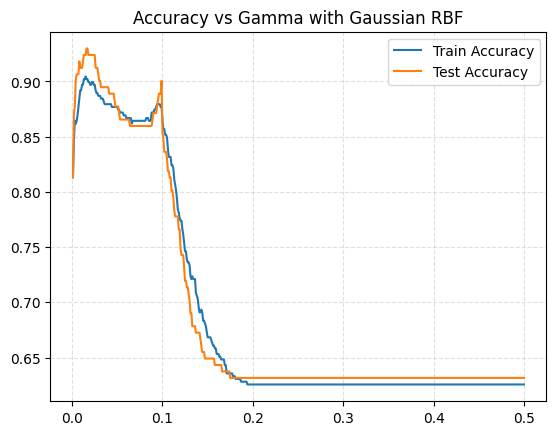
\includegraphics[width=0.5\linewidth]{img/GammaHyperparameterTuning.png}
    \caption{RBF Gamma tuning}
    \label{fig:gamma-tuning}
\end{figure}

Comparing the distribution of the values of the hidden layers in both
solutions, we can see that for $\gamma=0.015$ there is a wider range of
values, which have a less concentrated distribution, see Figure
\ref{fig:rbf-dist}.
\begin{figure}[H]
    \centering
    \centering
    \begin{subfigure}{0.45\linewidth}
        \centering
        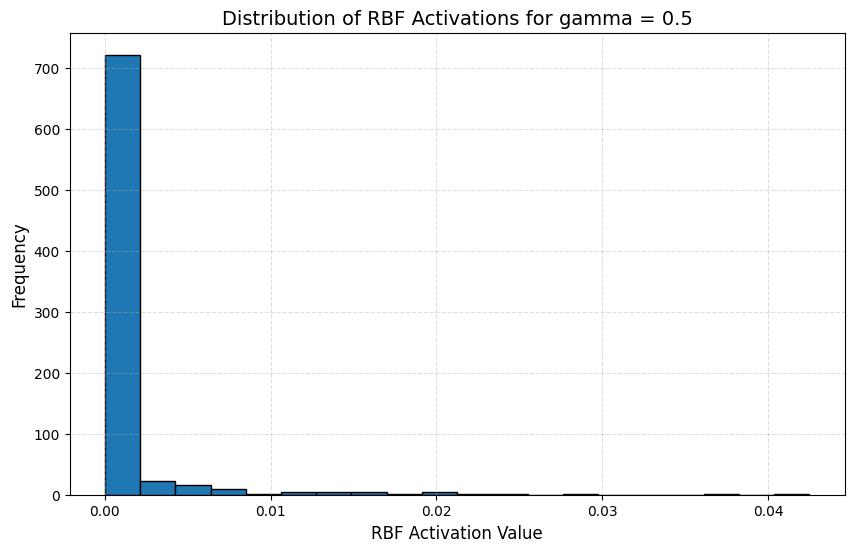
\includegraphics[width=\linewidth]{img/RBF_Activation_500.png}
        \caption{$\gamma=0.5$}
    \end{subfigure}
    \hfill % Add horizontal space between subfigures
    \begin{subfigure}{0.45\linewidth}
        \centering
        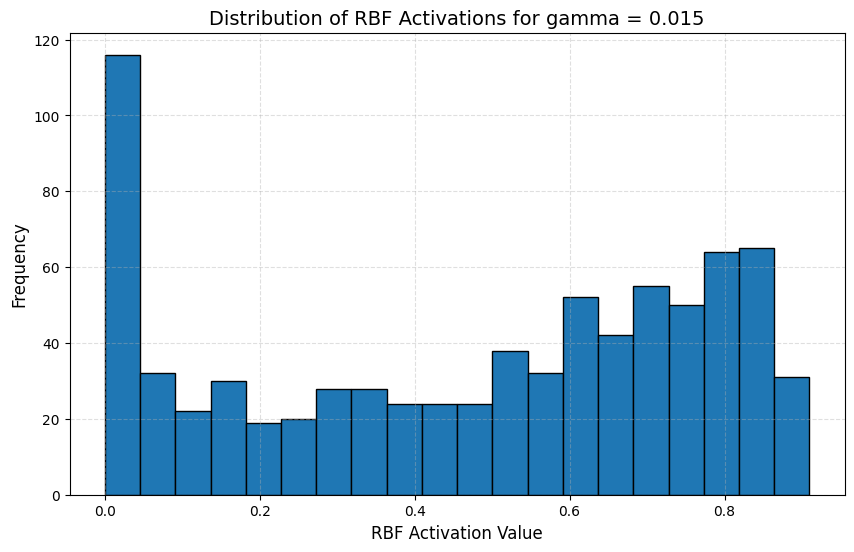
\includegraphics[width=\linewidth]{img/RBF_Activation_15.png}
        \caption{$\gamma=0.015$}
        \label{fig:rbf-dist-15}
    \end{subfigure}
    \caption{Hidden layer activation value distribution}
    \label{fig:rbf-dist}
\end{figure}

The distribution seen in Figure \ref{fig:rbf-dist-15} will allow
for a much more diverse activation for the output layer, but it
is still a skewed distribution, and the model is not able
to learn anything from observations that have RBF values
very close to zero for \textit{both} clusters, tuning the gamma value
is also expensive and something we want to avoid. Thus we considered
normalizing the values of the hidden layer before the logistic
regression. Making a Normalized Radial Basis Function Network.

\begin{figure}[H]
  \centering
  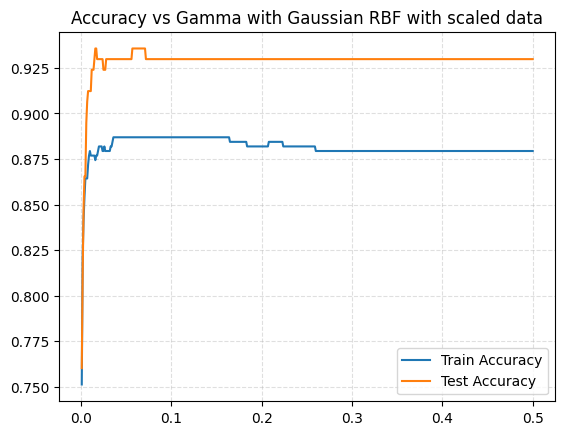
\includegraphics[width=0.5\linewidth]{img/NormGammaHyperparameterTuning.png}
  \caption{NRBF Gamma tuning}
  \label{fig:norm-gamma-tuning}
\end{figure}

This resulted on a much better testing accuracy, for $\gamma = 0.5$:
92.96\%, which is greater than the 92.4\% obtained in ex 4. and
additionally tuning the gamma stopped being a necessity, or effective at all.
If we do maximize train accuracy, we obtain the same 92.96\% test
accuracy.

Looking at the distributions we can see a much more balanced distribution,
since it is normalized, there are more activations, and the model can learn
more effectively.

\begin{figure}[H]
  \centering
  \centering
  \begin{subfigure}{0.45\linewidth}
      \centering
      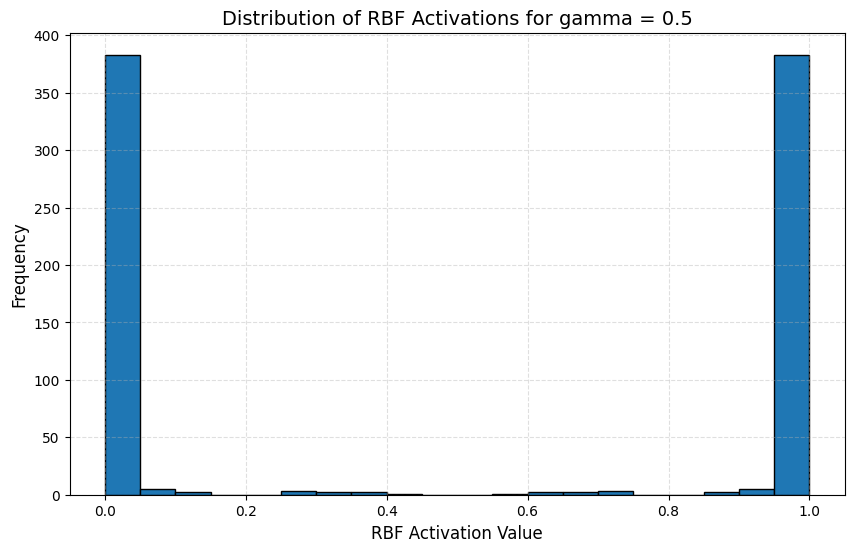
\includegraphics[width=\linewidth]{img/NRBF_Activation_500.png}
      \caption{$\gamma=0.5$}
  \end{subfigure}
  \hfill % Add horizontal space between subfigures
  \begin{subfigure}{0.45\linewidth}
      \centering
      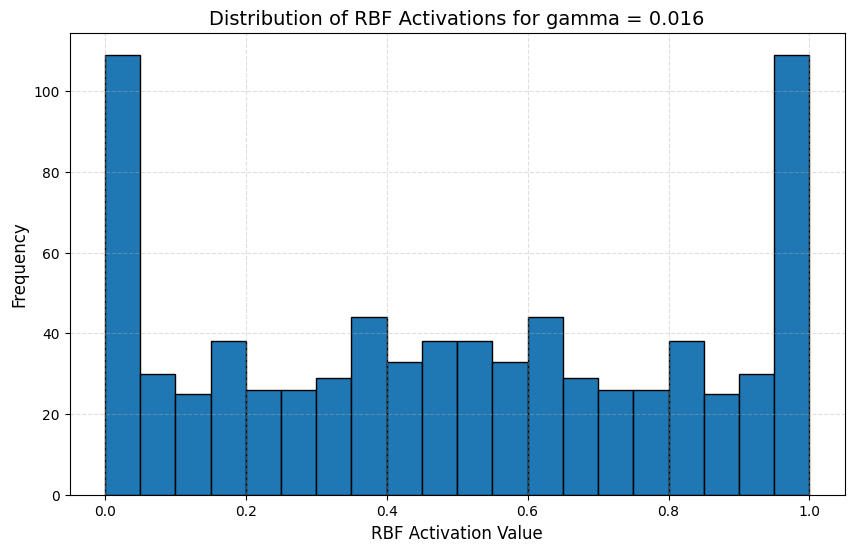
\includegraphics[width=\linewidth]{img/NRBF_Activation_16.png}
      \caption{$\gamma=0.036$}
      \label{fig:nrbf-dist-16}
  \end{subfigure}
  \caption{Hidden layer activation value distribution}
  \label{fig:nrbf-dist}
\end{figure}

However Gaussian is not the only effective function, Linear actually seems
to perform generally better, see Figure \ref{fig:linear-rbf}.

\begin{figure}[H]
  \centering
  \centering
  \begin{subfigure}{0.45\linewidth}
      \centering
      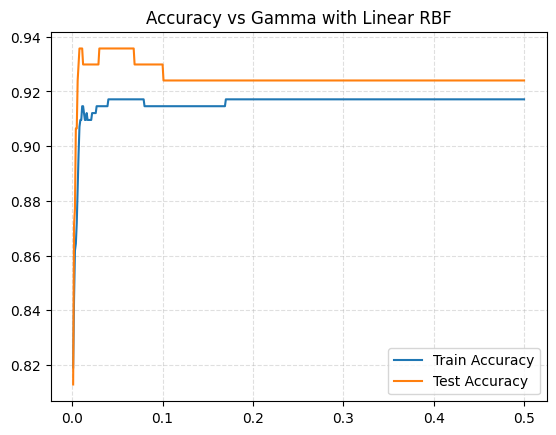
\includegraphics[width=\linewidth]{img/LinearRBF.png}
      \caption{Linear RBF}
  \end{subfigure}
  \hfill % Add horizontal space between subfigures
  \begin{subfigure}{0.45\linewidth}
      \centering
      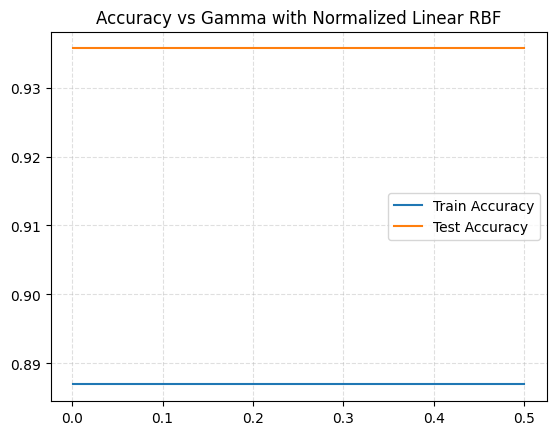
\includegraphics[width=\linewidth]{img/LinearNRBF.png}
      \caption{Normalized Linear RBF}
      \label{fig:nrbf-dist-16}
  \end{subfigure}
  \caption{Linear RBF Accuracy}
  \label{fig:linear-rbf}
\end{figure}

  \item \textit{Discuss your findings.}
\end{enumerate}

\newpage

\thispagestyle{empty}
\begin{thebibliography}{99}

\bibitem{journey} 
Luis Sa-Couto and Andreas Miroslaus Wichert, 
\textit{Machine Learning - A Journey To Deep Learning: With Exercises And Answers}, 
International series of monographs on physics, 
World Scientific Pub Co Inc, 2021, ISBN: 9789811234057.

\end{thebibliography}

% ----------------------------------------------------------------------
% Cover
% ----------------------------------------------------------------------

\end{document}

